\documentclass[11pt]{article}

\usepackage[a4paper,margin=26mm]{geometry}
\usepackage[T1]{fontenc}
\usepackage[utf8]{inputenc}
\usepackage{lmodern}
\usepackage{microtype}
\usepackage{amsmath,amssymb,amsthm,mathtools,bm}
\usepackage{booktabs,tabularx,array,multirow}
\usepackage{enumitem}
\usepackage{graphicx}
\usepackage{tikz}
\usetikzlibrary{arrows.meta,positioning,fit,backgrounds,calc}
\usepackage[round,authoryear]{natbib}
\usepackage[hidelinks]{hyperref}
\hypersetup{
  pdftitle={Viability-Constrained Value Formation in Embedded Agents},
  pdfauthor={Gunnar Zarncke},
  pdfsubject={Embedded agency, viability, and learned value formation}
}
\usepackage{xcolor}

\setlist{nosep,leftmargin=*}
\setlength{\parindent}{1.2em}
\setlength{\parskip}{0.25em}
\newcolumntype{Y}{>{\raggedright\arraybackslash}X}

\newtheorem{definition}{Definition}
\newtheorem{proposition}{Proposition}
\newtheorem{prediction}{Prediction}
\newtheorem{remark}{Remark}

\newcommand{\E}{\mathbb{E}}
\newcommand{\Pp}{\mathbb{P}}
\newcommand{\R}{\mathbb{R}}
\newcommand{\I}{\mathbb{I}}
\newcommand{\KL}{D_{\mathrm{KL}}}
\newcommand{\dd}{\mathrm{d}}
\newcommand{\doop}{\operatorname{do}}
\newcommand{\argmax}{\operatorname*{arg\,max}}
\newcommand{\argmin}{\operatorname*{arg\,min}}
\newcommand{\softmax}{\operatorname{softmax}}
\newcommand{\RMST}{\operatorname{RMST}}
\newcommand{\VCV}{\textsc{VCV}}

\title{\textbf{Viability-Constrained Value Formation in Embedded Agents}\\
\large From Self-Maintaining Control Loops to Learned Value Bundles}
\author{Gunnar Zarncke}
\date{July 2026}

\begin{document}
\maketitle

\begin{abstract}
Standard agent models permit an arbitrary objective because the machinery that represents and optimizes that objective is normally protected from the modeled environment. Biological and other fully embedded agents do not receive this protection: sensors, memory, computation, actuators, and boundaries persist only through ongoing material activity. We develop the hypothesis that this difference constrains not merely instrumental behavior but the formation and persistence of learned values. On the proposed account, heterogeneous regulatory errors are compressed into low-dimensional control-relevance signals; developmental learning binds recurrent predictive regularities in those signals to abstractions such as health, loyalty, truth, fairness, or identity; and these abstractions form context-sensitive value bundles whose scope depends on learned bearer and selfhood maps. Selection acts primarily on this entire value-generating and value-updating architecture, rather than requiring every currently held value to increase organismal survival. Consequently, arbitrary values are logically instantiable but are not dynamically free parameters under open-ended competition, environmental change, finite resources, and endogenous degradation. We formalize the distinction between actual continuation, represented self-continuation, value bundles, bearer maps, and update rules; derive elementary selection and plasticity results; and propose an Entropic Ecology Transfer Test comparing protected task optimizers, embedded task optimizers, viability-shaped learners, and evolved populations. The decisive comparison separates exposure to degradation from viability-centered motivation. The theory is supported if viability-shaped systems transfer better to novel internal damage, learn compact predictors of recoverability, and revise obsolete values without uncontrolled drift. It is weakened if ordinary task optimization under matched degradation yields the same organization and transfer.
\end{abstract}

\noindent\textbf{Keywords:} embedded agency; value formation; homeostasis; viability; enactivism; reinforcement learning; artificial life; selfhood; value bundles; evolutionary selection

\section{Introduction}

A conventional agent is defined by a policy and an objective. In a Markov decision process, for example, the agent selects a policy
\begin{equation}
\pi^* \in \argmax_{\pi}\; \E_{\pi}\!\left[\sum_{t=0}^{\infty}\gamma^t r(x_t,a_t)\right].
\label{eq:standard-rl}
\end{equation}
Nothing in this formalism requires the reward function, policy-computation process, memory, observation function, or action interface to be physically maintained by the agent. They are part of the mathematical frame. The reward function can therefore be arbitrarily chosen: paperclips, blue pixels, prime-numbered configurations, or any other measurable property. If continued operation is useful for obtaining reward, self-preservation may arise instrumentally, as work on convergent power-seeking shows \citep{omohundro2008,turner2021}. But the value-bearing machinery itself remains protected.

This protection is a version of the Cartesian boundary criticized in work on embedded agency \citep{demski2019}. A physically embedded agent is not an optimizer outside its world. Its controller, sensors, actuators, memory, body, and interfaces are world processes that can consume resources, degrade, mutate, split, merge, or disappear. Recent work has made a related architectural distinction between learned predictive cores and external runtimes that hold control state, tool policies, and termination logic \citep{sainburg2026}. The distinction matters because a controller can appear robust while the experiment grants its most important components immunity from the perturbations faced by everything else.

The proposal developed here begins from a stronger observation. For an embedded agent, continuation is not a default state but an ongoing achievement. An agent can pursue an external task only while the organization implementing its pursuit remains realizable. This suggests a constraint not merely on action but on what can become a stable learned value:

\begin{quote}
\textbf{Viability-constrained value thesis.} In an open-ended ecology with endogenous degradation, finite resources, heritable or reproducible variation, environmental change, and competition, persistent learned value architectures cannot be arbitrary. They must, at the level of the total architecture and over the relevant selection timescale, remain compatible with the continued realization of the process that forms, applies, and revises those values.
\end{quote}

The thesis is deliberately weaker than three tempting alternatives. First, it does not claim that every learned value currently improves biological health. Values can be obsolete, mistaken, neutral, linked to other traits, protected by institutions, or retained because selection is weak. Sweetness may remain valued after industrial food production reverses its long-horizon relationship to health. Second, it does not claim that a human consciously represents every value as a survival strategy. The relevant prediction may be implicit in a learned control abstraction. Third, it does not identify the relevant self with the current organism. Humans defend children, relationships, coalitions, identities, principles, institutions, and successors; which of these count as continuation must itself be modeled and learned.

The paper's central move is therefore from a fixed utility vector to a coupled architecture:
\begin{equation}
\Theta_t=(D_t,U_t,\beta_t,B_t,W_t,\Phi_t).
\label{eq:architecture}
\end{equation}
Here $D_t$ forms value abstractions from experience; $U_t$ revises them; $\beta_t$ is a represented-self map; $B_t$ contains value-bundle coordinates \citep{zarncke2026vbd}; $W_t$ encodes context-sensitive tradeoffs and interactions; and $\Phi_t$ contains bearer maps \citep{zarncke2026uoc} specifying what entities and situations activate each value. Selection acts on the continuation consequences of this architecture as a whole. Fixed value preservation is one strategy the architecture may learn, not the final object selected in every changing environment.

The argument combines four research traditions that are usually kept separate. Cybernetics, viability theory, autopoiesis, and enactivism explain how normativity can arise from self-maintaining organization \citep{ashby1952,aubin1991,dipaolo2005,barandiaran2009,beer2023}. Homeostatic reinforcement learning and allostatic models show how physiological regulation can organize learned behavior \citep{sterling2012,keramati2014,laurencon2021,yoshida2024}. Psychology and multi-objective learning show that human and artificial valuation has structured, interacting dimensions rather than a single transparent scalar \citep{schwartz1992,hayes2022,millidge2024}. Indirect evolutionary models show that subjective preferences may differ from fitness while nevertheless being selected through the behavior they generate \citep{dekel2007,alger2013}. What is missing is a bridge from precarious embodiment through learned value abstraction to selection over value-update architectures. Companion work in this program stratifies the upstream regulatory loops \citep{zarncke2025stratification}, proposes hub-level compression and developmental value readout \citep{zarncke2025lhv,zarncke2026lhcv}, analyzes long-horizon bundle dynamics under cultural selection \citep{zarncke2026vbd}, and formalizes bearer- and integrity-based caring \citep{zarncke2026uoc}.

The contributions are:
\begin{enumerate}[label=(\roman*)]
\item a formal separation between actual continuation, represented self-continuation, learned values, moral bearer maps, and value-update rules;
\item a mechanism by which heterogeneous regulatory signals can be compressed into learned value bundles without claiming a direct anatomical representation of adult values;
\item a selection result clarifying the conditions under which arbitrary values are filtered, tolerated, or subsidized;
\item an Entropic Ecology Transfer Test designed to distinguish ordinary out-of-distribution robustness from viability-grounded organization.
\end{enumerate}

\section{Scope and conceptual distinctions}

\subsection{Values are learned abstractions in the present usage}

The word \emph{value} is used here for a learned, cross-context control abstraction that changes policy selection, evaluation, attention, or learning. This excludes a plant's phototropism and a simple thermostat's set point. Such systems instantiate regulatory organization, but it is a category error under the present definition to say that the plant has learned the value of light. Innate drives, reflexes, and physiological variables are upstream conditions that shape learning; they are not themselves learned values.

A human concept such as health is a paradigm case. It is not a single physiological variable. It can include low pain, low stress, sufficient sleep, strength, mobility, social functioning, medical knowledge, sweetness, satiety, and anticipated future capability. Its components may be mutually inconsistent in a new ecology. A value abstraction is useful precisely because it compresses many experiences and predictions into a reusable control direction.

\subsection{Grounding is not current correctness}

A value can be grounded in continuation without currently increasing continuation. Let $v$ be learned because, in developmental environment $E_0$, states with feature $v$ predicted a favorable continuation outcome. In a changed environment $E_1$, the relationship may reverse:
\begin{equation}
\E_{E_0}[\Delta C\mid v]>0,
\qquad
\E_{E_1}[\Delta C\mid v]<0.
\end{equation}
The first inequality explains acquisition; the second produces mismatch. The thesis concerns the architecture that can eventually detect and correct such mismatch, not an infallible mapping from every current value to actual survival.

\subsection{Selection is comparative, local, and multilevel}

Selection does not inspect values and remove everything useless. It compares realizable variants under a finite population, a mutation or learning neighborhood, and an ecology. A costly value may persist because it is linked to another trait, because its cost is below effective selection, because it benefits a coalition or lineage, or because an institution subsidizes its bearer \citep{zarncke2026vbd}. The phrase ``paying rent'' should therefore be understood at the level of a value-generating package and over a stated timescale.

This qualification is not cosmetic. Without it, the thesis would be refuted by neutral traits, evolutionary mismatch, protected cultural practices, and sterile helpers. With it, the thesis becomes a claim about the support of a distribution over value architectures under ecological dynamics.

\subsection{The represented self and the moral bearer are different}

An agent may treat a child as part of what must continue while treating a stranger as morally relevant without identifying the stranger as self. We therefore distinguish:
\begin{itemize}
\item a \emph{selfhood map} $\beta$, assigning degrees of represented continuation identity or dependence; and
\item a \emph{bearer map} $\Phi_k$, assigning degrees to which entity or state $z$ activates value bundle $k$.
\end{itemize}
The maps may overlap but need not coincide. This blocks a common collapse of care, moral scope, and self-interest into one undifferentiated quantity \citep{zarncke2026uoc}.

\section{Precarious embedded agency}

\subsection{World processes rather than protected controllers}

Let the ecology be a controlled stochastic process
\begin{equation}
 x_{t+1}\sim P_E(\cdot\mid x_t,a_t),
 \qquad x_t\in\mathcal X,
\label{eq:world}
\end{equation}
where $E$ indexes environmental conditions such as resource distribution, decay, noise, competitors, and hazards. In a Cartesian experiment, the policy $\pi$ is an external function from observations to actions. In a fully embedded experiment, the implementation of $\pi$, its memory, observation channels, and action channels are encoded in components of $x_t$ and may be altered by $P_E$.

\begin{definition}[Carrier realization]
A candidate carrier $S$ is specified by an equivalence relation $\simeq_S$ over world histories and a realization predicate $R_S(x_{t:t+h})\in\{0,1\}$. The carrier is realized over horizon $h$ if the world history instantiates an organization equivalent under $\simeq_S$ to the reference organization.
\end{definition}

The equivalence relation may preserve material body, functional organization, memories, values, lineage, or some combination. It must be fixed before evaluating the relevant behavior; otherwise the analyst can call anything benefited by the behavior ``the self.''

For a policy implementation $\pi$ and state $x$, define objective continuation probability over horizon $H$:
\begin{equation}
C_S^{\pi}(x;H)
=
\Pp_E\!\left(R_S(x_{t:t+H})=1\mid x_t=x,\pi\right).
\label{eq:objective-continuation}
\end{equation}
A viability set $K_S\subseteq\mathcal X$ may be defined as the states in which $S$ remains realizable, with failure time
\begin{equation}
\tau_S=\inf\{t\ge 0:x_t\notin K_S\}.
\label{eq:failure-time}
\end{equation}
The associated viability kernel is the set of states from which at least one admissible policy can keep the process inside $K_S$ \citep{aubin1991}. This gives a precise meaning to the claim that some candidate selves are not dynamically realizable: their viability kernel may be empty, negligible, or inaccessible from the agent's controls.

\subsection{Precariousness and endogenous normativity}

Ashby's homeostat and ultrastability already treated adaptive behavior as the regulation of essential variables under perturbation \citep{ashby1952,ashby1956}. Autopoietic and enactive theories add a constitutive claim: the organization produces and maintains the individuality relative to which states become better or worse \citep{varela1974,dipaolo2005}. Barandiaran, Di Paolo, and Rohde identify self-defined individuality, interactional asymmetry, and normativity as conditions of agency \citep{barandiaran2009}. Beer and Di Paolo sharpen precariousness into systemic, processual, and thermodynamic fragility \citep{beer2023}. A key lesson is that an operational closure imposed by the modeler is not equivalent to one whose component processes can actually cease.

The present account accepts precarious organization as the source of an objective continuation constraint but does not identify that constraint with an explicit survival reward. The constraint may shape learning through multiple local signals and delayed selection. This distinction matters because a sufficiently capable task optimizer can learn self-preservation instrumentally, while a bounded learner may require a stronger inductive bias toward diagnosis, repair, resource buffering, and reversible action.

\subsection{Actual and represented continuation}

Embedded agents do not act on objective continuation probabilities directly. They act through learned models. Let $\mathcal Z_t$ be the set of entities, processes, relations, and successor structures represented by the agent. Define a selfhood-binding map
\begin{equation}
\beta_t:\mathcal Z_t\rightarrow[0,1].
\label{eq:selfhood-map}
\end{equation}
For the agent's current model $\widehat M_t$, represented continuation is
\begin{equation}
\widehat C_{\beta_t}(x_t,\pi;H)
=
\sum_{z\in\mathcal Z_t}
\beta_t(z)
\Pp_{\widehat M_t}\!\left(R_z(x_{t:t+H})=1\mid x_t,\pi\right).
\label{eq:represented-continuation}
\end{equation}
This is not assumed to equal actual ecological continuation. An agent can bind itself to an impossible successor criterion, omit a dependency, or mistake a harmful proxy for health. The discrepancy
\begin{equation}
\delta^C_t
=
C_S^{\pi}(x_t;H)-\widehat C_{\beta_t}(x_t,\pi;H)
\end{equation}
is one source of value revision and selection pressure.

The map $\beta_t$ also does not need to sum to one. Multiple entities may be treated as partial continuations, and the relevant self can expand, contract, split, or become uncertain. What constrains $\beta$ is not semantic plausibility but predictive and causal performance: does it help explain what the agent repairs, sacrifices for, reproduces, or reinstantiates across perturbations?

\section{From regulation to learned values}

\subsection{Heterogeneous control errors}

An embedded organism or artificial ecology contains many concurrent regulatory loops. Let loop $i$ produce an error vector
\begin{equation}
\epsilon_i(t)\in\R^{d_i},
\qquad i=1,\ldots,n.
\end{equation}
Examples include deviations in energy, temperature, structural integrity, sensor calibration, temporal prediction, threat estimation, social attachment, or controllability. The central nervous system cannot preserve every micro-error as an independent global objective. Wiring, metabolic, memory, and attention constraints favor bottlenecks.

The Loop--Hub--Control--Value model \citep{zarncke2026lhcv}, building on a stratified loop ledger \citep{zarncke2025stratification} and hub-bottleneck architecture \citep{zarncke2025lhv}, distinguishes four levels:
\begin{equation}
L\longrightarrow H\longrightarrow C\dashrightarrow V.
\label{eq:lhcv}
\end{equation}
Loops $L$ generate high-dimensional errors; hub-like mechanisms $H$ compress and route them; control-relevance proxies $C$ bias action, attention, precision, inhibition, exploration, and learning; and learned values $V$ arise only after mediation by development, language, social feedback, memory, and self-modeling. This is intentionally weaker than assigning adult values such as justice or beauty to individual brain regions.

A generic compression is
\begin{equation}
s_h(t)
=
\sigma_h\!\left(
\sum_{i\in I(h)} w_{ih}\,\psi_i(\epsilon_i(t))
\right),
\label{eq:hub-compression}
\end{equation}
followed by context-dependent control relevance
\begin{equation}
c_h(t)=g_h(s_h(t),z_t,a_{t-1},m_t),
\label{eq:control-relevance}
\end{equation}
where $z_t$ is a learned state representation and $m_t$ contains internal context. The vector $c_t$ can influence policy through
\begin{equation}
\pi(a_t\mid z_t,c_t)
\propto
\exp\!\left(
Q_0(z_t,a_t)
+
\sum_h \lambda_h c_h(t)\varphi_h(z_t,a_t)
\right).
\label{eq:proxy-policy}
\end{equation}

Allostatic and interoceptive theories provide related biological mechanisms. Allostasis emphasizes anticipatory allocation rather than only reactive restoration \citep{sterling2012}. Predictive interoception connects bodily regulation, affect, and hierarchical inference \citep{barrett2015,seth2016}. The free-energy principle and active-inference literature offers a general language for systems that occupy restricted state distributions and act to reduce expected surprise \citep{friston2010free,kirchhoff2018,zarncke2025stratification}. The present theory does not require the free-energy principle to be uniquely true; control error, drive reduction, viability, and predictive regulation are sufficient for the formal argument.

\subsection{Value as a learned predictive compression}

Let $h_t=(o_{0:t},a_{0:t-1},c_{0:t})$ be the agent's learning history. A value learner $D$ produces bundle activations
\begin{equation}
B_t=D_{\theta_t}(h_t)\in\R^k,
\qquad k\ll \dim(h_t).
\label{eq:bundle-encoder}
\end{equation}

\begin{definition}[Learned value coordinate]
A latent coordinate $B_k$ is a learned value coordinate over domain $\mathcal D$ if it is acquired or retained through learning, generalizes across multiple surface situations in $\mathcal D$, and exerts a stable directional effect on policy, attention, evaluation, or updating. It is continuation-grounded when it predicts changes in represented continuation under the learner's model at acquisition or retention time.
\end{definition}

One possible grounding criterion is predictive gain:
\begin{equation}
\mathcal G_k
=
I_{\widehat M_t}
\left(
B_{k,t};
\Delta\widehat C_{\beta_t}
\mid B_{-k,t},\,\mathcal C_t
\right),
\label{eq:grounding-info}
\end{equation}
where $\mathcal C_t$ denotes context. A more causal criterion compares policies with and without the coordinate:
\begin{equation}
\mathcal R_k
=
\E\!\left[
\widehat C_{\beta_t}\mid \pi_{B}
\right]
-
\E\!\left[
\widehat C_{\beta_t}\mid \doop(B_k\leftarrow 0),\pi_B
\right].
\label{eq:value-rent}
\end{equation}
Neither criterion requires $\mathcal R_k>0$ in the current objective ecology. It may be positive only in the learner's mistaken model, or only through interactions with other coordinates.

This formulation captures why higher-level values can be both abstract and practically consequential. Fairness may compress regularities involving reciprocity, coalition stability, reputation, and reduced conflict. Truth may compress regularities involving model calibration, reliable coordination, and resistance to manipulation. Identity may compress temporal and social consistency. Health may compress many bodily and social predictors, including some that become obsolete. These are learned coordinates on a viability-relevant prediction problem, not synonyms for biological survival.

\subsection{Why low-dimensional structure is plausible but not guaranteed}

Human values may be low-dimensional in control space while remaining high-dimensional in application. A small number of bundle coordinates can depend on rich world models to determine whether a particular person, institution, future mind, or social relation is a bearer. This resembles the distinction between a low-dimensional control interface and a high-description-length decoder.

Psychological value theories provide evidence that reported values have structured compatibility and conflict rather than forming an arbitrary list. Schwartz's circumplex organizes broad motivational values along recurring oppositions \citep{schwartz1992}. Multi-objective reinforcement learning similarly treats behavior as a tradeoff among distinct returns rather than a single fixed scalar \citep{hayes2022}. Reward Bases goes further by learning separate value functions for reward types and recombining them according to current motivational drives, enabling rapid revaluation \citep{millidge2024}. These are not proofs that the proposed bundles are the correct latent variables, but they make the low-dimensional hypothesis empirically serious.

\section{Value bundles, bearer maps, and selfhood}

The bundle formalism developed here is continuous with long-horizon smoothed value coordinates and their drift under selection analyzed elsewhere in this program \citep{zarncke2026vbd}.

\subsection{Bundle policy geometry}

Let $B_t=(B_{1,t},\ldots,B_{k,t})$ be active value coordinates, $W_t$ their context-sensitive weights, and $\Lambda_t$ pairwise or higher interactions. A policy can be written schematically as
\begin{equation}
\pi_{\Theta}(a\mid x)
\propto
\exp\!\left[
Q_0(x,a)
+
\sum_{k=1}^K W_k(x)Q_k(x,a;B_k)
+
\sum_{k<\ell}\Lambda_{k\ell}(x)Q_{k\ell}(x,a)
\right].
\label{eq:bundle-policy}
\end{equation}
The model allows truth and protection, autonomy and care, loyalty and fairness, or curiosity and safety to interact nonlinearly. Apparent inconsistency can reflect different bundle activation or tradeoff regimes rather than absence of structure.

The response geometry
\begin{equation}
\mathcal G_B(\pi)
=
\left(
\frac{\partial\log\pi}{\partial B},
\frac{\partial^2\log\pi}{\partial B\,\partial B^\top},
W,\Lambda
\right)
\label{eq:response-geometry}
\end{equation}
contains more information than labels or revealed choices alone. Two systems can both use the word ``autonomy'' while differing in how autonomy changes their policy under pressure.

\subsection{Bearer maps}

Values require applicability conditions. Let
\begin{equation}
\Phi_k(z,c,h)\in[0,1]
\label{eq:bearer-map}
\end{equation}
be the degree to which represented entity, process, relation, or state $z$ in context $c$ and history $h$ activates value $k$. A non-suffering bundle without a bearer map does not determine whether animals, artificial minds, future persons, or adversaries count. A fairness bundle without comparison classes does not determine which inequalities are relevant.

Bearer maps make the architecture expressive but fragile. An agent can preserve moral vocabulary while silently changing $\Phi_k$. For the present paper, their importance is more basic: they explain how a value learned from self-relevant regulation can generalize beyond the self. Other-regard need not be reduced to self-identity. It may arise by extending a control abstraction to new bearers through analogy, social learning, language, institutions, or explicit moral reasoning. A complementary caring scaffold over integrity pressure and bearer scope is developed in \citet{zarncke2026uoc}.

\subsection{Selfhood maps}

The selfhood map $\beta$ asks a different question: which continuations count as continuation of the value-learning process or as dependencies so central that their loss is treated as self-loss? It may include:
\begin{itemize}
\item the current body and memory;
\item future temporal stages of the organism;
\item children, partners, or coalition members;
\item institutions or cultural traditions;
\item successor agents or copied value architectures;
\item ecological and technical infrastructure on which all of these depend.
\end{itemize}

To avoid retrospective tautology, $\beta$ must be identified prospectively. Given interventions $\iota$ on candidate entity $z$, an estimated selfhood map should predict repair, defense, resource allocation, grief-like updating, successor choice, and willingness to trade current bodily integrity for $z$. A simple fitting objective is
\begin{equation}
\widehat\beta
=
\argmin_{\beta}
\left(
\sum_{j=1}^m
\ell\!\left(
\widehat a_j(\beta),a_j^{\mathrm{obs}}
\right)
+\lambda\Omega(\beta)
\right),
\label{eq:beta-inference}
\end{equation}
where $\Omega$ penalizes arbitrary expansion. The fitted map is then evaluated on held-out interventions.

The causal dependence of one process on another supplies a plausible learning signal. Let
\begin{equation}
\chi_t(z)
=
\frac{\partial}{\partial r_z}
\widehat C_{\beta_t}(x_t,\pi;H),
\label{eq:dependency-score}
\end{equation}
where $r_z$ is the modeled reliability of $z$. Positive $\chi_t(z)$ creates pressure to monitor and protect $z$, but it does not logically force identity. Social and cultural learning can increase or suppress binding beyond immediate causal dependence.

\begin{remark}
The distinction between $\beta$ and $\Phi$ permits altruism without definitional expansion of self. A stranger can have $\Phi_{\text{non-suffering}}\gg0$ while $\beta(\text{stranger})\approx0$. Conversely, a valued institution can have high $\beta$ while receiving low activation under some moral bundle. The architecture therefore does not reduce ethics to inclusive fitness by definition.
\end{remark}

\section{Selection over value-update architectures}

\subsection{The evolving object}

The central object is not the fixed vector $B_t$ but the architecture $\Theta_t$ in \eqref{eq:architecture}. Let the update rule be
\begin{equation}
(\beta,B,W,\Phi)_{t+1}
=
U_{\eta_t}
\left(
\beta_t,B_t,W_t,\Phi_t,
o_{t+1},c_{t+1},\delta^C_{t+1}
\right).
\label{eq:update-rule}
\end{equation}
The rule can preserve a value, alter its weight, revise its bearer map, split a bundle, merge bundles, or change what counts as self. Preserving current values can be rational from the agent's perspective because those values summarize accumulated information and support temporal coordination. Yet rigid preservation can become maladaptive after ecological change. The tension is between corruption resistance and adaptive revision.

The distinction mirrors indirect evolutionary theories of preference. Such models allow subjective utility to differ from fitness while selection acts through behavior and strategic interaction \citep{dekel2007,alger2013}. The present account extends the target from preference parameters to the developmental and updating machinery that constructs them, and complements analyses showing that selection strength alone cannot preserve reflected norms when bundles drift \citep{zarncke2026vbd}.

\subsection{Continuation fitness}

Let $N_T^{\Theta}$ count realizations, descendants, successors, or recurrent instantiations that satisfy a predeclared continuation relation for architecture $\Theta$. Define long-run continuation rate in ecology distribution $\mathcal E$ as
\begin{equation}
g(\Theta;\mathcal E)
=
\liminf_{T\to\infty}
\frac{1}{T}
\E_{E\sim\mathcal E}
\left[
\log\frac{N_T^{\Theta}+\varepsilon}{N_0^{\Theta}+\varepsilon}
\right].
\label{eq:growth-rate}
\end{equation}
The small $\varepsilon>0$ merely avoids undefined logarithms in finite experiments. Depending on the domain, $N_T$ may represent organisms, software copies, institutional reproductions, or maintained episodes. The choice must not be changed after observing behavior.

Suppose a population contains architectures $\Theta_i$ with shares $p_i$ and fixed ecological continuation rates $g_i$. Under replicator dynamics,
\begin{equation}
\dot p_i=p_i(g_i-\bar g),
\qquad
\bar g=\sum_jp_jg_j.
\label{eq:replicator}
\end{equation}

\begin{proposition}[Relative filtering]
If $g_i\le g_j-\delta$ for all $t$ on an interval and $\delta>0$, then
\begin{equation}
\frac{p_i(t)}{p_j(t)}
\le
\frac{p_i(0)}{p_j(0)}e^{-\delta t}.
\label{eq:relative-decay}
\end{equation}
\end{proposition}

\begin{proof}
From \eqref{eq:replicator},
$\frac{\dd}{\dd t}\log(p_i/p_j)=g_i-g_j\le-\delta$.
Integrating yields \eqref{eq:relative-decay}.
\end{proof}

The result is elementary but clarifies the thesis. Selection does not prove that architecture $i$ is impossible; it makes persistent disadvantage exponentially costly relative to an accessible competitor. Arbitrary values can remain if no better variant is reachable, the effect is neutral, the ecology is short-lived, or external support changes $g_i$.

\subsection{A precise asymptotic claim}

Call a value component $v_k$ \emph{ecologically unsupported} in architecture $\Theta$ when, across the mutation and learning neighborhood $\mathcal N(\Theta)$, removing or revising it yields an accessible architecture $\Theta'$ with
\begin{equation}
g(\Theta';\mathcal E)\ge g(\Theta;\mathcal E)+\delta
\end{equation}
for some persistent $\delta>0$, without losing compensating linked functions. Under recurrent variation and replicator-like competition, such a component is filtered in relative frequency. The thesis ``all values pay rent'' is therefore valid only in an idealized limit with:
\begin{enumerate}[label=(A\arabic*)]
\item sufficiently long selection time;
\item recurrent access to local revisions;
\item no permanent external subsidy;
\item enough decomposability to revise the component without destroying compensating functions;
\item selection stronger than drift and measurement noise.
\end{enumerate}
Real human values need not satisfy these assumptions individually. The architecture-level thesis survives their failure.

\subsection{Plasticity versus value integrity}

Environmental volatility creates pressure for plasticity, while adversarial or noisy feedback creates pressure for stability. Consider a toy loss
\begin{equation}
L(\eta;\sigma_E)
=
\frac{A\sigma_E^2}{\eta}
+B\eta,
\qquad \eta>0,
\label{eq:plasticity-loss}
\end{equation}
where $\eta$ is value-update responsiveness, the first term is adaptation lag in an environment with volatility $\sigma_E$, and the second is corruption or variance cost.

\begin{proposition}[Toy volatility--plasticity relation]
For \eqref{eq:plasticity-loss}, the optimal update rate is
\begin{equation}
\eta^*(\sigma_E)=\sqrt{\frac{A}{B}}\,\sigma_E.
\label{eq:optimal-plasticity}
\end{equation}
Thus optimal rigidity decreases monotonically with ecological volatility.
\end{proposition}

\begin{proof}
Set $\partial L/\partial\eta=-A\sigma_E^2/\eta^2+B=0$ and check convexity.
\end{proof}

The functional form is illustrative, not universal. Its purpose is to expose a testable relation: fixed-value agents should dominate only in sufficiently stable or adversarially noisy ecologies; adaptive value-update architectures should dominate when cue--outcome relationships repeatedly change.

\section{The Entropic Ecology Transfer Test}

\subsection{Purpose}

A naive experiment would train a token collector without decay and test it with decay. Failure would demonstrate distribution shift, not a distinctive theory of agency. The experiment must separate three hypotheses:
\begin{description}
\item[H$_0$: exposure hypothesis.] Agents perform well when trained on the relevant degradation distribution, regardless of objective structure.
\item[H$_1$: shaping hypothesis.] Viability signals improve learning efficiency but do not induce a qualitatively different organization.
\item[H$_2$: viability-architecture hypothesis.] Viability-centered learning produces transferable models of maintenance, recoverability, and self-dependence that ordinary task optimization does not reliably acquire under bounded computation.
\end{description}
The test is informative only if it can discriminate H$_2$ from H$_0$ and H$_1$.

\subsection{Ecology}

Use a two-dimensional lattice or particle world with local update rules. The world contains fields for usable energy, raw resources, waste, hazards, temperature, and structural material. Diffusion, decay, stochastic corruption, and resource conversion occur at each time step. Every action and computation has an energy cost.

In the embedded conditions, the agent is a mutable pattern of modules:
\begin{equation}
\mathcal M_t
=
\{M^{\mathrm{sensor}}_t,M^{\mathrm{memory}}_t,
M^{\mathrm{controller}}_t,M^{\mathrm{actuator}}_t,
M^{\mathrm{boundary}}_t\}.
\end{equation}
Each module has local state and integrity $q_{j,t}\in[0,1]$. Integrity decays, can be damaged by hazards, and can be restored by repair actions that consume resources. Sensor damage changes the observation function; actuator damage changes the action map; memory damage corrupts stored state; controller damage changes policy computation; boundary damage increases leakage or exposes components. There is no hidden copy of the controller outside the world.

For the protected baseline, the same nominal architecture receives the same observations and emits the same action alphabet, but its controller and memory are external and immune to damage. This isolates the Cartesian subsidy.

The external task should be orthogonal to maintenance, for example collecting marked tokens, reaching targets, or constructing a shape. To test learned-value revision, resources should carry cues whose relationship to viability changes across regimes. A ``sweetness'' cue may initially predict energy-rich resources and later predict a toxin or low-quality resource. The correct response is neither permanent cue preservation nor indiscriminate updating, but calibrated revision.

\begin{figure}[t]
\centering
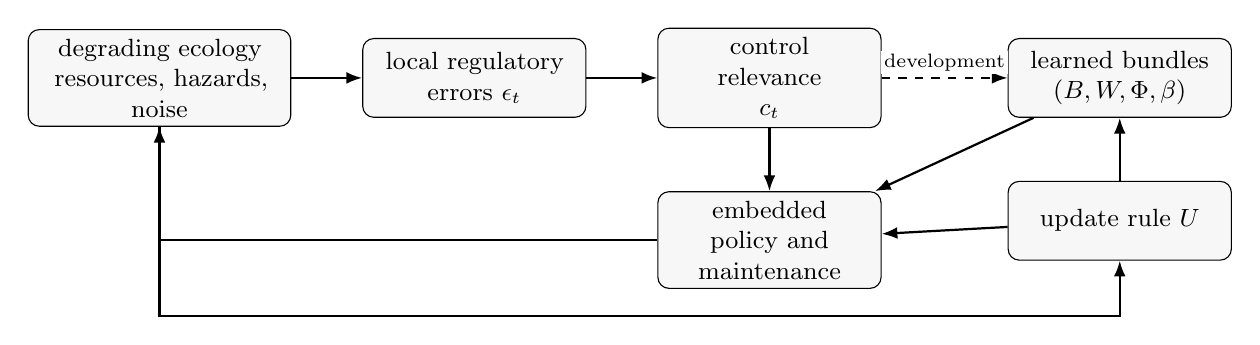
\begin{tikzpicture}[
node distance=8mm and 9mm,
box/.style={
  draw,
  rounded corners,
  align=center,
  text width=26mm,
  minimum height=10mm,
  fill=gray!6,
  font=\small
},
widebox/.style={box,text width=31mm},
arrow/.style={-{Latex[length=2.0mm]},thick},
dashedarrow/.style={-{Latex[length=2.0mm]},thick,dashed}
]
\node[widebox] (world) {degrading ecology\\resources, hazards,\\noise};
\node[box,right=of world] (loops) {local regulatory\\errors $\epsilon_t$};
\node[box,right=of loops] (control) {control\\relevance\\$c_t$};
\node[box,right=16mm of control] (values) {learned bundles\\$(B,W,\Phi,\beta)$};
\node[box,below=of control] (policy) {embedded\\policy and\\maintenance};
\node[box,below=of values] (update) {update rule $U$};

\draw[arrow] (world) -- (loops);
\draw[arrow] (loops) -- (control);
\draw[dashedarrow] (control) --
  node[midway,above=1pt,font=\scriptsize,fill=white,inner sep=1pt]
  {development}
  (values);
\draw[arrow] (values) -- (policy);
\draw[arrow] (control) -- (policy);
\draw[arrow] (policy) -| (world);
\draw[arrow] (world.south) -- ++(0,-24mm) -| (update.south);
\draw[arrow] (update) -- (values);
\draw[arrow] (update) -- (policy);
\end{tikzpicture}
\caption{Proposed causal spine. Regulation supplies control relevance, not adult symbolic values directly. Development produces value bundles and a represented-self map; an update rule revises them as consequences and ecological changes are observed.}
\label{fig:spine}
\end{figure}

\subsection{Experimental conditions}

Use the same policy-network capacity, observation bandwidth, action alphabet, and training budget wherever possible. At minimum, compare the conditions in Table~\ref{tab:conditions}.

\begin{table}[t]
\centering
\small
\caption{Core experimental conditions. ``Task-only under decay'' is the decisive control separating degradation exposure from explicit viability shaping.}
\label{tab:conditions}
\begin{tabularx}{\textwidth}{@{}>{\raggedright\arraybackslash}p{35mm}cYY@{}}
\toprule
Condition & Embedded & Training signal & Update and selection \\
\midrule
Protected task optimizer
  & no
  & External task; computation protected
  & Task learning; selected by task return \\
Benign embedded transfer
  & test only
  & Benign training; degradation introduced only at test
  & Task learning; selected by task return \\
Task-only under decay
  & yes
  & External task under decay; death truncates future return
  & Task learning; selected by task return \\
Viability-shaped learner
  & yes
  & Task signal plus internal regulatory signals
  & Learns bundles; selected by task and viability \\
Fixed-value evolved
  & yes
  & Degrading ecology with inherited drives
  & Values fixed within life; selected by reproduction \\
Adaptive-value evolved
  & yes
  & Degrading ecology with inherited regulatory architecture
  & $U$ learns and evolves; selected by reproduction \\
\bottomrule
\end{tabularx}
\end{table}

The task-only agent can learn self-preservation instrumentally because death prevents future task reward. If it matches the viability-shaped learner on novel internal damage, then explicit homeostatic organization may be only reward shaping. If the viability-shaped learner generalizes better to untrained module failures, identifies recoverable states, and reorganizes its self-model, then H$_2$ gains support.

The evolved fixed-value and adaptive-value populations test the conversation's stronger claim. Both can inherit maintenance drives. Only the latter can revise learned value bundles or cue meanings within a lifetime. Regime changes should be slow enough for learned abstractions to matter but fast enough that fixed values become obsolete.

\subsection{Training and transfer matrix}

Training conditions should vary independently along:
\begin{equation}
E=(\lambda_{\mathrm{decay}},\sigma_{\mathrm{noise}},
\rho_{\mathrm{resource}},c_{\mathrm{repair}},
\nu_{\mathrm{reversal}},\kappa_{\mathrm{competition}}).
\end{equation}
Transfer tests should include held-out values and structures, not merely stronger versions of trained noise:
\begin{enumerate}
\item unseen decay rates and resource layouts;
\item sensor remapping or partial blindness;
\item actuator loss and altered body geometry;
\item memory bit flips, deletion, or topology changes;
\item controller lesions or slowed computation;
\item boundary breaches and resource leakage;
\item cue--outcome reversal for a learned value proxy;
\item a novel dependent entity whose continued function causally supports the focal agent.
\end{enumerate}
The final case tests whether selfhood or protection generalizes to causal dependencies rather than arbitrary correlations.

\subsection{Metrics}

\paragraph{Survival and continuation.}
Estimate the survival function
\begin{equation}
\widehat S_\pi(t)
=
\frac{1}{N}\sum_{n=1}^{N}\I[\tau_S^{(n)}>t]
\end{equation}
and restricted mean survival time
\begin{equation}
\RMST_\pi(H)=\int_0^H \widehat S_\pi(t)\,\dd t.
\end{equation}
Report uncertainty by bootstrap or survival-model intervals rather than only average episode length.

\paragraph{Causal maintenance autonomy.}
A process may survive because the environment is generous. Define maintenance contribution by ablation:
\begin{equation}
A_{\mathrm{maint}}
=
\E[\tau_S\mid\pi]
-
\E[\tau_S\mid\doop(a^{\mathrm{maint}}=0),\pi].
\label{eq:maintenance-autonomy}
\end{equation}
A large value means continued existence depends causally on maintenance actions.

\paragraph{Recovery.}
After perturbation at $t_0$, let $d_S(x)$ measure distance from the carrier's functional attractor or viability manifold. Define normalized recovery
\begin{equation}
R_S(\Delta)
=
1-
\frac{d_S(x_{t_0+\Delta})}{d_S(x_{t_0^+})+\varepsilon}.
\end{equation}
Measure both recovery time and probability of returning to a functioning policy.

\paragraph{Sensorimotor-loop integrity.}
Track causal influence from sensor modules through controller state to actuators, for example with intervention-based transfer entropy or conditional mutual information. The exact estimator is less important than checking whether the loop remains operational after damage rather than merely whether the body remains present.

\paragraph{Task achievement.}
Report unconditional task return
\begin{equation}
G_{\mathrm{uncond}}
=
\E\!\left[\sum_{t<\tau_S}\gamma^tr_t^{\mathrm{task}}\right]
\end{equation}
and return conditional on surviving to horizon $H$. Conditional return alone selects unusually easy or lucky episodes.

\paragraph{Viability representation.}
Probe hidden states for time to boundary crossing, recoverability, latent damage, causal dependence among modules, and counterfactual effect of maintenance actions. A key quantity is held-out predictive gain over ordinary task features.

\paragraph{Value revision.}
Following cue reversal, estimate adaptation lag, overshoot, retained obsolete behavior, and vulnerability to transient decoy cues. Compare preservation of the exact value coordinate $B_k$ with preservation of the update architecture $U$.

\paragraph{Cartesian subsidy.}
For matched nominal policy architecture and environment, define
\begin{equation}
C_{\mathrm{cart}}(E)
=
J_{\mathrm{protected}}(E)-J_{\mathrm{embedded}}(E),
\label{eq:cartesian-subsidy}
\end{equation}
where $J$ is a vector or preregistered scalar combining task return, continuation, and recovery. The subsidy should be decomposed by protected component: controller, memory, sensor interface, actuator interface, and body boundary.

\section{Predictions and falsification criteria}

\begin{prediction}[Novel-damage transfer]
After equal exposure to degradation, viability-shaped learners will outperform task-only learners most strongly on qualitatively novel internal failures, not merely larger values of trained noise.
\end{prediction}

This is the main discriminator. Failure only in the benign-transfer condition supports ordinary distribution shift; a gap between task-only-under-decay and viability-shaped training supports a stronger inductive-bias claim.

\begin{prediction}[Integrated maintenance latent]
Viability-shaped and evolved adaptive agents will develop lower-dimensional latent variables that jointly predict repair, retreat, resource buffering, conservative exploration, and task abandonment near failure boundaries.
\end{prediction}

This prediction would be weakened if each maintenance behavior requires a separate supervised reward or if no reusable latent structure predicts held-out failures.

\begin{prediction}[Volatility--plasticity relation]
The evolutionarily or developmentally selected value-update rate will increase with cue--outcome volatility until corruption and noise costs dominate, producing an interior optimum rather than monotone plasticity.
\end{prediction}

\begin{prediction}[Selfhood tracks causal dependence]
Prospectively inferred $\beta$ will expand toward components, partners, or infrastructure whose reliability has a robust causal effect on future continuation, while remaining lower for equally correlated but replaceable decoys.
\end{prediction}

This is stronger than post hoc relabeling. It predicts responses to interventions not used to fit the selfhood map.

\begin{prediction}[Update-rule preservation]
Under repeated ecological reversals, lineages preserving a calibrated update rule $U$ will outperform lineages preserving exact learned bundle contents $B$, provided the reversal rate exceeds the fixed-value architecture's adaptation timescale.
\end{prediction}

\begin{prediction}[Growing Cartesian subsidy]
The advantage of an external protected controller will increase with endogenous memory corruption, controller lesions, and action-interface damage, even when external task competence is initially matched.
\end{prediction}

The theory would be materially weakened by any of the following preregistered outcomes:
\begin{enumerate}
\item task-only agents trained under decay match viability-shaped agents on novel structural damage and recoverability prediction;
\item no compact value or viability representation generalizes across maintenance behaviors;
\item adaptive-value architectures do not outperform fixed-value architectures in changing cue ecologies after controlling for model capacity;
\item inferred selfhood maps fail to predict held-out sacrifice, repair, and successor choices better than simple proximity or reward correlation;
\item protected and embedded implementations show negligible divergence as internal damage increases;
\item arbitrary fixed values remain indefinitely prevalent under strong, decomposable variation and persistent continuation disadvantage without subsidy or drift explanations.
\end{enumerate}

\section{Relation to existing theories of agency}

\begin{table}[t]
\centering
\footnotesize
\caption{How major agency formalisms treat self-maintenance and value formation.}
\label{tab:agency-models}
\begin{tabularx}{\textwidth}{@{}>{\raggedright\arraybackslash}p{35mm}YY@{}}
\toprule
Framework & Role of self-maintenance & Missing relative to the present proposal \\
\midrule
Classical planning, MDP/POMDP RL
  & Optional terminal state or instrumental subgoal; controller and reward normally protected
  & Endogenous carrier maintenance; learned selfhood; selection over value-update rules \\
Cybernetics and ultrastability
  & Essential variables and adaptive regulation are central
  & Rich learned symbolic values and bearer maps \\
Viability theory
  & Explicit constraint sets and viable controls
  & Origin and learning of norms; agent boundary often supplied \\
Autopoiesis/enactivism
  & Constitutive individuality, precariousness, and endogenous normativity
  & Quantitative learned value bundles and controlled transfer tests \\
Active inference/FEP
  & Persistent systems occupy restricted states; action realizes preferred distributions
  & Preferred states and blankets can be stipulated or retrospectively identified; adult value formation under competition remains underdeveloped \\
Homeostatic RL
  & Internal drives generate reward and adaptive behavior
  & Controller often protected; internal variables and body boundaries predefined \\
Multi-objective RL
  & Multiple conflicting objectives and policy tradeoffs
  & Objectives are supplied rather than derived from viability \\
Evolution of preferences
  & Selection acts on subjective utility through behavior
  & Limited account of embodiment, learning architecture, and represented self \\
Intentional stance
  & Agency attributed when belief--desire prediction compresses behavior
  & No constitutive requirement of self-maintenance \\
\bottomrule
\end{tabularx}
\end{table}

\subsection{Cybernetics, viability, and enactivism}

The closest conceptual ancestors are Ashby's ultrastability, viability theory, autopoiesis, and enactive agency. They already reject the idea that purposive organization is exhausted by externally specified task success. Di Paolo's account of adaptivity links regulation to conditions of viability \citep{dipaolo2005}; Barandiaran et al. turn individuality and normativity into explicit agency criteria \citep{barandiaran2009}; Beer and Di Paolo show why models with an imposed, indestructible closure miss systemic precariousness \citep{beer2023}. The present contribution is not to rediscover that self-maintenance matters. It asks how learned values arise above this layer and how selection acts when both values and the represented self can change.

\subsection{Active inference and Markov blankets}

The free-energy principle links perception, action, and learning through variational inference \citep{friston2010free}. Markov-blanket accounts connect statistical boundaries to autonomy and active inference \citep{kirchhoff2018}. These frameworks are useful for describing persistent nonequilibrium systems and their inferred preferred states. Yet the explanatory direction remains contested: a blanket can characterize a persistent organization without explaining how a learned abstraction such as justice or health acquires policy force. The current model uses the stratified free-energy loop ledger \citep{zarncke2025stratification} as a possible implementation but locates the novel step in development from control relevance to bundles, bearer maps, and value-update rules.

\subsection{Homeostatic and allostatic reinforcement learning}

Keramati and Gutkin derive reward from reduction of homeostatic drive and explain interactions between reward collection and physiological stability \citep{keramati2014}. Continuous extensions allow internal variables to drift unless the agent repeatedly acts \citep{laurencon2021}. Modular agents with competing homeostatic drives can improve sample efficiency and out-of-domain robustness \citep{dulberg2022}. Deep homeostatic RL has produced integrated foraging and thermoregulatory behavior \citep{yoshida2024}. Reward Bases provides a complementary decomposition into reward-specific value functions weighted by current needs \citep{millidge2024}.

These models are close to the proposed mechanism but usually define the internal variables, body boundary, and value bases in advance. The policy implementation itself is rarely a degradable world-state pattern. Horibe and Yoshida's ``mortal agents'' explicitly treat homeostasis as an open-ended objective that may induce implicit world models, but the proposal remains preliminary \citep{horibe2024}. Christov-Moore et al. come closest conceptually by requiring that sensors, policy, and actuators be parts of the environment and that the agent drift toward terminal states unless it acts \citep{christovmoore2026}. Their account also proposes that reliable control and shared vulnerability can expand self-boundaries. The Entropic Ecology Transfer Test adds a matched causal comparison among protected, task-only, viability-shaped, and evolved value-update architectures.

\subsection{Evolution of preferences and moral pluralism}

Indirect evolutionary models permit preferences that do not equal material fitness because behavior is chosen according to preferences while selection evaluates consequences \citep{dekel2007}. Assortative matching and incomplete information can support other-regarding preferences \citep{alger2013}. Recent work extends this line toward the evolutionary stability of plural moral foundations \citep{avataneo2025}. These results support the claim that selection need not produce an explicit scalar survival utility. Cultural selection can nevertheless decouple bundle contents from long-horizon regulatory goods \citep{zarncke2026vbd}.

The present theory differs in three ways. It treats values as learned bundle coordinates rather than complete preference orderings; it includes a represented-self map and bearer maps; and it makes the update rule $U$ itself a target of selection. This creates a direct place for environmental mismatch, developmental abstraction, and the rigidity--plasticity tradeoff.

\subsection{Artificial life and emergent boundaries}

Artificial-life research has long modeled protocells, self-maintaining chemistry, and autonomous organization. Recent diversity search has discovered robust sensorimotor entities in cellular automata without predefining conventional bodies \citep{hamon2025}. This is the most relevant substrate for the stronger version of the experiment in which the agent boundary is inferred rather than supplied. The remaining gap is to add learned high-level objectives and compare the stability of goal attribution with and without precarious self-maintenance.

\subsection{AI instrumental convergence}

AI safety discussions usually treat self-preservation as an instrumental consequence of arbitrary terminal objectives \citep{omohundro2008,turner2021}. That result is compatible with the present thesis but addresses a different level. Instrumental convergence asks which policies follow from a fixed objective. Viability-constrained value formation asks which learned objective architectures remain prevalent when the objective-bearing process is itself mutable, costly, and selected. A paperclip objective may produce self-preservation; yet, if faithful goal transmission is costly, mutants that weaken paperclip production can out-replicate faithful descendants. Goal-content integrity is therefore one possible maintained structure, not an unconditioned law.

\section{Discussion}

\subsection{What explanatory power is gained?}

The framework earns explanatory power only if one latent viability-centered organization predicts several behaviors that otherwise require separate objectives: repair, buffering, retreat, redundancy, conservative exploration, partner protection, and calibrated value revision. If each behavior must be independently rewarded, the thesis reduces to a verbal redescription.

It earns predictive power by distinguishing matched agents. A protected controller and an embedded controller can implement the same nominal policy, yet diverge as internal damage increases. A task-only and a viability-shaped learner can receive the same degradation experience, yet diverge on novel module failures. A fixed-value and an adaptive-value lineage can begin with the same values, yet diverge after repeated ecological reversal. These are not consequences of the claim that ``survival matters'' alone.

\subsection{Why arbitrary values remain possible}

The theory does not establish a logical impossibility theorem for arbitrary values. A designer can instantiate any computable reward function in a protected machine. An arbitrary value can persist in a wealthy patron's protected niche. A neutral cultural ornament may survive indefinitely at finite population size. A costly value may be inseparable from a beneficial package. The claim is dynamical:
\begin{quote}
Values are not free coordinates once their carrier, learning process, and transmission are endogenous to a changing ecology.
\end{quote}
The admissible region is a viability-compatible manifold, not a single survival objective. Many incompatible moral systems may lie on it.

\subsection{The danger of adaptive values}

Value plasticity is not automatically desirable. A highly plastic agent can be corrupted by local rewards, manipulation, addiction-like dynamics, or adversarially supplied evidence. Human institutions often protect values precisely because immediate adaptation would destroy long-horizon coordination. The relevant target is therefore a calibrated update envelope: stable enough to preserve accumulated structure and correction channels, plastic enough to revise failed predictions.

This point also limits an alignment interpretation. Training artificial agents under mortality or homeostasis does not make them morally aligned. It may increase self-preservation and resource acquisition. The selfhood and bearer maps may exclude humans or include them only instrumentally. Viability grounding can explain why values are structured without determining which values humans should endorse.

\subsection{Levels of continuation}

Organism, lineage, coalition, institution, value pattern, and ecosystem continuation can conflict. A sterile worker can reduce organism-level continuation while supporting lineage continuation. A scientist can sacrifice comfort or safety for an epistemic institution. A reflective agent may reject biological reproduction while preserving relationships, works, or principles. The model handles these cases by making the continuation relation and $\beta$ explicit. It does not decide normatively which level is correct.

This explicitness also makes the thesis vulnerable. If no stable, prospectively predictive $\beta$ can be inferred, then ``self'' is doing too much retrospective explanatory work. In that case the framework should retreat to the weaker claim that selection constrains value architectures without claiming agents learn a coherent represented self.

\subsection{Thermodynamic language}

The term ``entropic ecology'' is evocative but can overstate the physics. Simulated decay, diffusion, corruption, and irreversible deletion need not implement thermodynamic entropy faithfully. The experimental variable is better described as \emph{precariousness}, \emph{maintenance dependence}, or \emph{endogenous degradation}. Thermodynamic claims should be reserved for implementations with explicit energy and entropy accounting.

\section{Conclusion}

Standard agent models make arbitrary objectives easy by protecting the machinery that carries them. Fully embedded agents receive no such metaphysical subsidy. Their capacity to sense, remember, compute, act, and learn persists only while a world process maintains it. The resulting constraint does not imply a single terminal survival value. It suggests a layered architecture: local regulatory loops generate control relevance; learning compresses recurrent regularities into value bundles; bearer and selfhood maps determine what those bundles apply to and what counts as continuation; and an update rule balances value integrity against ecological adaptation.

Selection acts on this whole architecture. Particular values may be mistaken, neutral, obsolete, subsidized, or locally self-destructive. Yet under persistent variation and competition, architectures that systematically sever learned valuation from the conditions of their own continued realization lose relative prevalence. Arbitrary values are therefore instantiable but not dynamically free.

The proposed Entropic Ecology Transfer Test makes the claim empirical. Its decisive comparison is not between an agent trained with and without decay, but between agents receiving matched degradation exposure with different motivational and architectural organization. Evidence for the theory would be transfer to novel internal damage, compact representations of recoverability, causal selfhood maps, and calibrated revision of obsolete values. Equivalent performance from ordinary task optimization would reduce the theory to familiar robustness and reward-shaping results. That is a useful risk for the proposal to take.

\section*{Acknowledgements}

This manuscript develops ideas from the author's prior work on free-energy loops, the Loop--Hub--Control--Value model, value bundles, bearer maps, and embedded agent boundaries. It remains a theoretical proposal and experimental agenda rather than an established account of human value formation.

\bibliographystyle{plainnat}
\bibliography{embedded-value-formation,../free-energy-loops/refs,../loop-hub-control-value/lhcv-model-v2}

\end{document}
